\documentclass[runningheads,a4paper]{llncs}

\usepackage[utf8]{inputenc}
\usepackage[T1]{fontenc}

\usepackage{textcomp}
\usepackage{listings}
\lstset{frame=lines,captionpos=b,numberbychapter=false,escapechar=§,basicstyle=\ttfamily,upquote=true}

\usepackage[activate=compatibility]{microtype}
\usepackage{graphicx}

% autoref command
\usepackage[pdftex,urlcolor=black,colorlinks=true,linkcolor=black,citecolor=black]{hyperref}
\def\sectionautorefname{Section}
\def\subsectionautorefname{Subsection}
\def\figureautorefname{Fig.}

% todo macro
\usepackage{color}
\newcommand{\todo}[1]{\noindent\textcolor{red}{{\bf \{TODO}: #1{\bf \}}}}

\usepackage{xspace}
\newcommand{\googleplus}{Google\nolinebreak\hspace{0em}\raisebox{.28ex}{\tiny\bf +}\kern-0.2ex\xspace}

\hyphenation{}

\usepackage{comment}
% \linespread{0.96}

\begin{document}

\title{SEKI@home, or Crowdsourcing\\ a~Google Knowledge Graph API}
\titlerunning{SEKI@home, or Crowdsourcing a~Google Knowledge Graph API}
\authorrunning{T. Steiner and S. Mirea}

\author{
  Thomas Steiner\inst{1}\thanks{Full disclosure: T. Steiner is also a~Google employee, S. Mirea a~Google intern.} \and
  Stefan Mirea\inst{2}
}

\institute{Universitat Politècnica de Catalunya -- Department LSI,
		   Barcelona, Spain\\
		   \urldef{\emails}\UrlFont\path|tsteiner@lsi.upc.edu|
		   \emails\rm \and
		   Computer Science, Jacobs University Bremen, Germany\\
		   \urldef{\emails}\UrlFont\path|s.mirea@jacobs-university.de|
		   \emails\rm
}

\maketitle
% Start footnotes again by 0.
\setcounter{footnote}{0}

\begin{abstract}
In May 2012, the Web search engine Google has introduced the so-called Knowledge Graph,
a~graph that understands real-world entities and their relationships to one another.
It currently contains more than 500 million objects,
as well as more than 3.5 billion facts about
and relationships between these different objects.
Soon after its announcement, people started to ask
for a~Knowledge Graph Application Programming Interface (API),
however, as of today, Google does not provide one.
With \emph{SEKI@home}, which stands for \emph{Search for Embedded Knowledge Items},
we propose a~browser extension-based approach to crowdsource such an API.
As people with the extension installed search on Google.com,
the extension sends anonymous Knowledge Graph facts from Search Engine Results Pages (SERPs)
to a~centralized, publicly accessible triple store,
and thus over time recreates an open Knowledge Graph.
We have implemented and made available a~prototype browser extension
tailored to the Google Knowledge Graph, however,
note that the concept of \emph{SEKI@home} is generalizable for other closed knowledge bases.
\end{abstract}

\section{Introduction}

\subsection{The Google Knowledge Graph}
With the introduction of the Knowledge Graph, the search engine Google
has made a~significant paradigm shift towards \textit{``things, not strings''}~\cite{singhal2012_1},
as a~post on the official Google blog states.
Entities covered by the Knowledge Graph include landmarks, celebrities, cities, sports
teams, buildings, movies, celestial objects, works of art, and more.
The Knowledge Graph enhances Google search in three main ways:
by disambiguation of search queries,
by search log-based summarization of key facts,
and by explorative search suggestions.
This triggered demand for a~Knowledge Graph API that would allow for
programmatically accessing the facts stored in the Knowledge Graph~\cite{quora2012}.
At time of writing, however, no such API is available.

\subsection{On Crowdsourcing} \label{sec:on-crowdsourcing}
The term \emph{crowdsourcing} was first coined by Jeff Howe
in an article in the magazine Wired~\cite{howe2006}.
It is a~\textit{portmanteau} of ``crowd'' and ``outsourcing''.
Howe writes: \textit{``The new pool of cheap labor:
everyday people using their spare cycles to create content, solve problems,
even do corporate R\&D''}.
The difference to outsourcing is that the crowd is undefined by design.
We suggest crowdsourcing for the described task of extracting facts from
SERPs with Knowledge Graph results for two reasons:
\textit{(i)} there is no publicly available list
of the 500 million objects~\cite{singhal2012_1} in the Knowledge Graph, and
\textit{(ii)} even if there was such a~list,
it would not be practicable (nor allowed by the terms and conditions of Google)
to crawl it.

\subsection{Search Results as Social Media}
Kaplan and Haenlein have defined social media as
\textit{``a~group of Internet-based applications that build on the ideological and
technological foundations of Web 2.0, and that allow the creation and
exchange of user-generated content''}~\cite{kaplan2010}.
We argue that search results are social media as well,
especially in the case of Google with its tight integration of \googleplus,
a~feature called \emph{Search plus Your World}~\cite{singhal2012_2}.

\subsection{Contributions and Paper Structure}
In this position paper, we describe and provide a~prototype implementation
of an approach, tentatively titled \emph{SEKI@home} and
based on crowdsourcing via a~browser extension,
to make closed knowledge bases programmatically and openly accessible.
We demonstrate its applicability with the Google Knowledge Graph.
The extension can be added to the Google Chrome browser via \todo{Add Chrome Web Store URL},
our unofficial crowdsourced Google Knowledge Graph API can be tested at
\todo{Add API URL}.

The remainder of this paper is structured as follows:
\todo{Add Paper Structure}

\section{Related Work}
Wrappers around Web services or Web pages have been used in the past
to lift data from the original source to a~meaningful, machine-readable RDF level.
Examples are the Google Art wrapper by Guéret~\cite{gueret2011},
which lifts the data from the Google Art project~\cite{sood2011},
or the now discontinued SlideShare wrapper\footnote{\url{http://linkeddata.few.vu.nl/slideshare/}} by the same author.
Such wrappers typically work by mimicking the URI scheme of the site they are wrapping.
Adapting parts of the URL of the original resource for that of the wrapper
provides access to the desired data.
Wrappers do not offer SPARQL endpoints, as their data gets computed on-the-fly.

With \emph{SEKI@home}, we offer a~related, however, still different in the detail,
approach to lift and make machine-readably accessible
closed datasets like the Knowledge Graph.
The entirety of the dataset being unknown,
via crowdsourcing, we can distribute the heavy burden
of crawling the whole Knowledge Graph on many shoulders.
Finally, by storing the extracted facts centrally in a~triple store,
our approach allows for openly accessing the data via the standard SPARQL protocol.

\section{Methodology}
\subsection{Browser Extensions}
We have implemented our prototype browser extension for the Google Chrome browser.
Chrome extensions are small software programs that users can install
to enrich their browsing experience.
Via so-called \emph{content scripts},
extensions can inject and modify the contents of Web pages.
We have implemented an extension that gets activated when a~user
uses Google to search the Web.

\subsection{Web Scraping}
Web scraping is a~technique to extract data from Web pages.
We use CSS selectors~\cite{hunt2012} to retrieve page content from SERPs
that have an associated real-world entity in the Knowledge Graph.
An exemplary query selector is \texttt{.kno-desc}
(all elements with class name ``kno-desc''),
which via the JavaScript command \texttt{document.querySelector}
returns the description of a~Knowledge Graph entity.

\subsection{Lifting the Extracted Knowledge Graph Data}
Albeit the claim of the Knowledge Graph is
\textit{``things, not strings''}~\cite{singhal2012_1},
what gets displayed to search engine users are strings,
as can be seen in \autoref{fig:screenshot}.
In order to make this data meaningful again, we need to lift it.
We use JSON-LD~\cite{sporny2012}, a~JSON representation format
for expressing directed graphs;
mixing both Linked Data and non-Linked Data in a~single document.
JSON-LD allows for adding meaning by simply including or referencing a~context.
The syntax is designed to not disturb already deployed systems running on JSON,
but provide a~smooth upgrade path from JSON to JSON-LD.

\begin{figure}[htb!]
  \begin{center}
   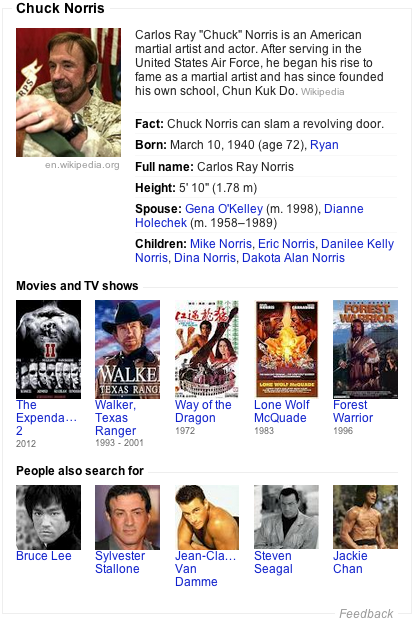
\includegraphics[width=0.5\linewidth]{./screenshot.png}
  \end{center}  
  \caption{Google Knowledge Graph result for the real-world entity \emph{Chuck Norris}.}
  \label{fig:screenshot}
\end{figure}

We have modeled the plaintext Knowledge Graph terms (or predicates)
like ``Born'', ``Full name'', ``Height'', ``Spouse'', etc.
in the special namespace \texttt{gkg} (for Google Knowledge Graph)
that has already been partially mapped to common Linked Data vocabularies.
One example is \texttt{gkg:Description},
which directly maps to \texttt{dbpprop:shortDescription} from DBpedia.
Similar to the unknown list of objects in the Knowledge Graph (see \autoref{sec:on-crowdsourcing}),
there is no known list of Knowledge Graph terms,
which makes a~complete mapping impossible.
We have collected \todo{Add Number of Collected Knowledge Graph Terms} Knowledge Graph terms
as of time of writing, however, the mapping to Linked Data terms
will be a~permanent work in progress.
\autoref{code:jsonld} shows the lifted, meaningful JSON-LD as returned by the extension.

\begin{lstlisting}[caption=Subset of the meaningful JSON-LD from the Chuck Norris Knowledge Graph data. The mapping of the Knowledge Graph terms can be seen in the @context., label=code:jsonld, float=bth!, escapechar=§]
{
  "@id": "http://openknowledgegraph.org/data/H4sIAAAAA[...]",
  "@context": {
    "Name": "http://xmlns.com/foaf/0.1/name",
    "Topic_Of": {
      "@id": "http://xmlns.com/foaf/0.1/isPrimaryTopicOf",
      "type": "@id"
    },
    "Fact": "http://openknowledegraph.org/ontology/Fact",
    "Query": "http://openknowledegraph.org/ontology/Query",
    "Full_name": "http://xmlns.com/foaf/0.1/givenName",
    "Height": "http://dbpedia.org/ontology/height",
    "Spouse": "http://dbpedia.org/ontology/spouse"
  },
  "Topic_Of": "http://en.wikipedia.org/wiki/Chuck_Norris",
  "Name": "Chuck Norris",
  "Fact": ["Chuck Norris can cut thru a knife w/ butter."],
  "Full_name": ["Carlos Ray Norris"],
  "Height": ["5' 10\""],
  "Spouse": [
    {
      "@id": "http://openknowledgegraph.org/data/H4sIA[...]",
      "Query": "gena o'kelley",
      "Name": "Gena O'Kelley"
    },
    {
      "@id": "http://openknowledgegraph.org/data/H4sIA[...]",
      "Query": "dianne holechek",
      "Name": "Dianne Holechek"
    }
  ]
}
\end{lstlisting} 

\section{Evaluation}

\section{Future Work}

\section{Conclusion}
In this paper, we have shown a~generalizable approach
to first opening up closed datasets by means of crowdsourcing,
and then making the extracted facts universally and openly accessible.
As an example dataset, we have used the Google Knowledge Graph.
The extracted facts can be accessed via the standard SPARQL protocol
from the Google-independent Open Knowledge Graph website
(\url{http://openknowledgegraph.org/sparql}).
Just like datasets evolve over time, the Knowledge Graph in concrete,
the facts extracted via the \emph{SEKI@home} approach as well
mirror those changes eventually.
Granted that provenance of the extracted data is handled appropriately,
we hope to have contributed a~useful socially enabled chain link
to the Linked Data world.

\section*{Acknowledgments}
%\small
T. Steiner is partially supported by the European Commission
under Grant No.~248296 FP7 (\mbox{I-SEARCH} project).

%\linespread{1}
\bibliographystyle{abbrv}
\bibliography{iswc2012}

\end{document}